\documentclass[a4paper,14pt]{extarticle}

% Путь до папки с общими шаблонами
\newcommand{\pathToCommonFolder}{/home/denilai/Desktop/LaTeX/Common}
% Название работы в титуле
\newcommand{\workname}{Практическая работа №1}
% Название дисциплины в титуле
\newcommand{\discipline}{Программирование на языке Python}

% Вставка заготовки преамбулы
% Этот шаблон документа разработан в 2014 году
% Данилом Фёдоровых (danil@fedorovykh.ru) 
% для использования в курсе 
% <<Документы и презентации в \LaTeX>>, записанном НИУ ВШЭ
% для Coursera.org: http://coursera.org/course/latex .
% Исходная версия шаблона --- 
% https://www.writelatex.com/coursera/latex/5.3

% В этом документе преамбула

% Для корректного использования русских символов в формулах
% пакеты hyperref и настройки, связанные с ним, стоит загуржать
% перед загрузкой пакета mathtext



% поддержка русских букв
% кодировка шрифта
%\usepackage[T2A]{fontenc} 
\usepackage{pscyr}

% использование ненумеровонного абзаца с добавлением его в содержаниеl

\newcommand{\anonsection}[1]{\section*{#1}\addcontentsline{toc}{section}{#1}}
\newcommand{\sectionunderl}[1]{\section*{\underline{#1}}}


% настройка окружения enumerate
\usepackage{enumitem}
\setlist{noitemsep}
\setlist[enumerate]{labelsep=*, leftmargin=1.5pc}

\usepackage{hyperref}

% сначала ставить \usepackage{extsizes} % Возможность сделать 14-й шрифт
% для корректной установки полей вставлять преамбулу следует в последнюю очередь (но перед дерективой замены \rmdefault)
\usepackage[top=20mm,bottom=25mm,left=35mm,right=20mm]{geometry} % Простой способ задавать поля

\hypersetup{				% Гиперссылки
	unicode=true,           % русские буквы в раздела PDF
	pdftitle={Заголовок},   % Заголовок
	pdfauthor={Автор},      % Автор
	pdfsubject={Тема},      % Тема
	pdfcreator={Создатель}, % Создатель
	pdfproducer={Производитель}, % Производитель
	pdfkeywords={keyword1} {key2} {key3}, % Ключевые слова
	colorlinks=true,       	% false: ссылки в рамках; true: цветные ссылки
	linkcolor=red,          % внутренние ссылки
	citecolor=black,        % на библиографию
	filecolor=magenta,      % на файлы
	urlcolor=blue           % на URL
}

%%% Работа с русским языком
\usepackage{cmap}					% поиск в PDF
\usepackage{mathtext} 				% русские буквы в формулах
\usepackage[T2A]{fontenc}			% кодировка
\usepackage[utf8]{inputenc}			% кодировка исходного текста
\usepackage[english,russian]{babel}	% локализация и переносы
\usepackage{indentfirst}
\frenchspacing

%для изменения названия списка иллюстраций
\usepackage{tocloft}


\renewcommand{\epsilon}{\ensuremath{\varepsilon}}
\renewcommand{\phi}{\ensuremath{\varphi}}
\renewcommand{\kappa}{\ensuremath{\varkappa}}
\renewcommand{\le}{\ensuremath{\leqslant}}
\renewcommand{\leq}{\ensuremath{\leqslant}}
\renewcommand{\ge}{\ensuremath{\geqslant}}
\renewcommand{\geq}{\ensuremath{\geqslant}}
\renewcommand{\emptyset}{\varnothing}

% Изменения параметров списка иллюстраций
\renewcommand{\cftfigfont}{Рисунок } % добавляем везде "Рисунок" перед номером
\addto\captionsrussian{\renewcommand\listfigurename{Список иллюстративного материала}}

\newcommand{\tm}{\texttrademark\ }
\newcommand{\reg}{\textregistered\ }


%%% Дополнительная работа с математикой
\usepackage{amsmath,amsfonts,amssymb,amsthm,mathtools} % AMS
\usepackage{icomma} % "Умная" запятая: $0,2$ --- число, $0, 2$ --- перечисление

%% Номера формул
%\mathtoolsset{showonlyrefs=true} % Показывать номера только у тех формул, на которые есть \eqref{} в тексте.
%\usepackage{leqno} % Нумереация формул слева

%% Свои команды
\DeclareMathOperator{\sgn}{\mathop{sgn}}

%% Перенос знаков в формулах (по Львовскому)
\newcommand*{\hm}[1]{#1\nobreak\discretionary{}
{\hbox{$\mathsurround=0pt #1$}}{}}


% отступ для первого абзаца главы или параграфа
%\usepackage{indentfirst}

%%% Работа с картинками
\usepackage{graphicx}  % Для вставки рисунков
\graphicspath{{images/}{screnshots/}}  % папки с картинками
\DeclareGraphicsExtensions{.pdf,.png,.jpg}
\setlength\fboxsep{3pt} % Отступ рамки \fbox{} от рисунка
\setlength\fboxrule{1pt} % Толщина линий рамки \fbox{}
\usepackage{wrapfig} % Обтекание рисунков текстом

%%% Работа с таблицами
\usepackage{array,tabularx,tabulary,booktabs} % Дополнительная работа с таблицами
\usepackage{longtable}  % Длинные таблицы
\usepackage{multirow} % Слияние строк в таблице

%%% Теоремы
\theoremstyle{plain} % Это стиль по умолчанию, его можно не переопределять.
\newtheorem{theorem}{Теорема}[section]
\newtheorem{proposition}[theorem]{Утверждение}

\theoremstyle{plain} % Это стиль по умолчанию, его можно не переопределять.
\newtheorem{work}{Практическая работа}[part]


 
 
\theoremstyle{definition} % "Определение"
\newtheorem{corollary}{Следствие}[theorem]
\newtheorem{problem}{Задача}[section]
 
\theoremstyle{remark} % "Примечание"
\newtheorem*{nonum}{Решение}



%%% Программирование
\usepackage{etoolbox} % логические операторы

%%% Страница

%	\usepackage{fancyhdr} % Колонтитулы
% 	\pagestyle{fancy}
%   \renewcommand{\headrulewidth}{0pt}  % Толщина линейки, отчеркивающей верхний колонтитул
% 	\lfoot{Нижний левый}
% 	\rfoot{Нижний правый}
% 	\rhead{Верхний правый}
% 	\chead{Верхний в центре}
% 	\lhead{Верхний левый}
%	\cfoot{Нижний в центре} % По умолчанию здесь номер страницы

\usepackage{setspace} % Интерлиньяж
\onehalfspacing % Интерлиньяж 1.5
%\doublespacing % Интерлиньяж 2
%\singlespacing % Интерлиньяж 1

\usepackage{lastpage} % Узнать, сколько всего страниц в документе.

\usepackage{soul} % Модификаторы начертания


\usepackage[usenames,dvipsnames,svgnames,table,rgb]{xcolor}


\usepackage{csquotes} % Еще инструменты для ссылок

%\usepackage[style=authoryear,maxcitenames=2,backend=biber,sorting=nty]{biblatex}

\usepackage{multicol} % Несколько колонок

\usepackage{tikz} % Работа с графикой
\usepackage{pgfplots}
\usepackage{pgfplotstable}

% модуль для вставки рыбы
\usepackage{blindtext}

\usepackage{listings}
\usepackage{color}


% для поворота отдельной страницы. Использовать окружение \landscape
\usepackage{pdflscape} 
\usepackage{rotating} 


\definecolor{mygreen}{rgb}{0,0.6,0}
\definecolor{mygray}{rgb}{0.5,0.5,0.5}
\definecolor{mymauve}{rgb}{0.58,0,0.82}


% пример импорта файла
%\lstinputlisting{/home/denilai/repomy/conf/distributions}

\lstset{
	language=Python,
	basicstyle=\footnotesize,        % the size of the fonts that are used for the code
	numbers=left,                    % where to put the line-numbers; possible values are (none, left, right)
	numbersep=5pt,                   % how far the line-numbers are from the code
	numberstyle=\tiny\color{mygray}, % the style that is used for the line-numbers
	stepnumber=2,                    % the step between two line-numbers. If it's 1, each line will be numbered
	% Tab - 2 пробела
	tabsize=2,    
	% Автоматический перенос строк
	breaklines=true,
	frame=single,
	breakatwhitespace=true,
	title=\lstname 
}



% установка размера шрифта для всего документа
%\fontsize{20pt}{18pt}\selectfont
%\usepackage{extsizes} % Возможность сделать 14-й шрифт

\author{Кирилл Денисов}
\title{Практическая работа №2}
\date{\today}

% установка полуторного интервала
% \usepackage{setspace}  
% \onehalfspacing

% использовать Times New Roman
\renewcommand{\rmdefault}{ftm}

\begin{document}
\thispagestyle{empty}

% Вставка первого титульного листа
%\newcounter{withouttheme}

%\setcounter{withouttheme}{<n>} установить значение счетчика  withouttheme для определения, нужна ли тема
%    {0} - нужна
%    {1} - не нужна

%\setcounter{withoutsubmissiondate}{<n>} установить значение счетчика  withoutsubmissiondate для определения, нужна ли дата представления к защите
%     {0} - нужна
%     {1} - не нужена
\begin{center}
	\begin{figure}[h!]
		\begin{center}
		%\vspace{-10ex}
		
\includegraphics[width=0.17\linewidth]{\pathToCommonFolder/gerb}
		%\caption{}\label{pic:first}
		%	\vspace{5ex}
		\end{center}	
	\end{figure}
 	\small	МИНОБРНАУКИ РОССИИ \\
	Федеральное государственное бюджетное образовательное учреждение\\
						высшего образования\\
\normalsize					
\textbf{«МИРЭА – Российский технологический университет»\\
						РТУ МИРЭА}\\
						\noindent\rule{1\linewidth}{1pt}\\
       Институт информационных технологий\\ %\vspace{2ex}
					\kafedra\\
		\vspace{3ex}
			\large \textbf{\workname}  \\
		%\vspace{1ex}
						по дисциплине\\ «\discipline» \\
		\vspace{3ex}
		\ifnum \value{withouttheme}=0 {
			\textbf{Тема работы:}\\ <<\theme>>
		}
		\else {}
		\fi
\vspace{10ex}
\small
\begin{table}[h!]
\begin{tabular}{lp{0.6\linewidth}l}
	\textbf{Выполнил:} & студент группы ИВБО-02-19 & \\ 
	& & \studentfio \\%Д.~Н.~Федосеев\\%А.~М.~Сосунов\\%К.~Ю.~Денисов\\%И.~А.~Кремнев
	\textbf{Принял:} & \rang & \\
	& & \teacherfio \hfill\\
\end{tabular}
\end{table}
\end{center}
\ifnum \value{withoutsubmissiondate}=0 {
	\begin{flushleft}
		Работа представлена к защите <<\rule{3ex}{1pt}>>\rule{10ex}{1pt} 202\rule{1ex}{1pt} г.\hfill
	\end{flushleft}
\else {}
\fi

\normalsize
\begin{center}	
\vfill
Москва 2022
\end{center}


\newpage


\section{Практическое занятие №1. Вариант №6}
Цель работы: изучить синтаксис языка программирования \textit{Pyhton}, изучить синтаксис условных операторов, операторов ветвления и математических операторов.


\begin{problem} Реализовать функцию
\[f(x,y,z) = \sin y - 36y^2+\frac{\cos{67x^6-z^5-89}+\frac{z^6}{36}}{\cos x-81x^6+36} - \sqrt{ \frac{\cos z + 19x^8-19}{z^3 - y^2-94} }. \]
\end{problem}
\begin{nonum}
Для реализации данной функции воспользуемся стандартными математическими операторами и функциями языка \textit{Python}.


\vspace{2ex}

\begin{lstlisting}
def simple (x,y) :
	return (x**4 + x)**2 - 69*y**8 -math.sqrt((x/8 - 86*x**4)/(math.sin(x) +x**3 - 24)) - ((y**8 + math.exp(x))/(x**5 - math.log(y)))

\end{lstlisting}
\vspace{3ex}

Примеры вычисления $simple$:
\begin{enumerate}
	\item $simple(75,‐13,‐90) = ‐4.84e+13$
	\item $simple(21,47,‐39) = ‐3.22e+11$
\end{enumerate}

\end{nonum}

\begin{problem} Реализовать кусочно-линейную функцию
	\[
	f(x) = 
		\begin{cases}
			27\left(\cos x + \sin x\right)^4 + 91x^6,&\text{если }x < 188;\\
			x^3 + 49x^8,& \text{если }188\le x < 247;\\
			96x^7 -76x^5,& \text{если }247 \le x < 285;\\
			x^3 - \cos x -78,& \text{если }285 \le x < 384;\\
			x + x^3 + 5,& \text{если } x \ge 384.
		\end{cases}
	\]
\end{problem}
\newpage
\begin{nonum}
	Для решения данной задачи используем условный оператор \textit {if}	
	\begin{lstlisting}
	def piecewise (x) :
		if x < -9 :
			return x**8 + 37*x**5 + 31
		if x >= -9 and x < 59:
			return x**3 - math.log(x) - 90
		if x >= 59 and x < 83:
			return (92*x**6 + math.sin(x) - 39)**4 - 59*x**5
		if x >= 83:
			return 67*(x**8) - x**2
	\end{lstlisting}
		
Примеры вычисления $piecewise:$
\begin{enumerate}
	\item $piecewise(124) =  6.55e+18$
	\item $piecewise(116) = 2.22e+14$
\end{enumerate}	
\end{nonum}

\begin{problem}
	Реализовать итерационную функцию
	\[
		f(n)= 51 \sum_{i=1}^{n} \left(27i^3+i^7\right) - \sum_{i=1}^{n} \left(e^i+\frac{i^5}{68}\right).
	\]
\end{problem}

\begin{nonum}
	Для реализации данной итерационной функции используем операторы цикла \textit{for in range}
	%\newpage
	\vspace{3ex}
	\begin{lstlisting}
	def iterate (n,m):
		acc1 = 0
		acc2 = 0
		for i in range(1,n+1):
			for j in range(1,m+1):
				acc1 += j**3 + 37*j**4 + 31
		for i in range(1,n+1):
			acc2 += math.cos(i) + math.log(i)
		return 60*acc1 + 43*acc2
	\end{lstlisting}
	
	Примеры вычисления $iterate$:
	\begin{enumerate}
		\item $iterate(45) = ‐5.53e+19$
		\item $iterate(50) = ‐8.20e+21$
	\end{enumerate}
\end{nonum}
\begin{problem}	
	Реализовать рекуррентную функцию
	\begin{align*}
		f(0) &= 10,\\
		f(1) &= 5, \\
		f(n) &= \frac 1 {86} f(n-1) - \cos {f(n-2)}
	\end{align*}
	\begin{nonum}
		Для реализации рекуррентной функциии прибегнем к рекурсивному вызову разрабатываемой функции.
		\vspace{3ex}
		\begin{lstlisting}
			def recursion (x):
				if x == 0: return 6
				if x == 1: return 10
			return math.tan(recursion(x-1)) - 1/30*recursion(x-2)**2
		\end{lstlisting}
		\vspace{3ex}
		
		Примеры вычисления $recursion(x)$:
		\begin{enumerate}
			\item $recursion(16) = ‐7.31e‐01$
			\item $recursion(14) = -7.63e-01$
		\end{enumerate}
	\end{nonum}
	
\end{problem}
\newpage

\section{Практическая работа №2. Вариант 6}
\begin{problem}
	Реализовать функцию--дерево решений
	\begin{figure}[h!]
		\begin{center}
			%\vspace{-5ex}
			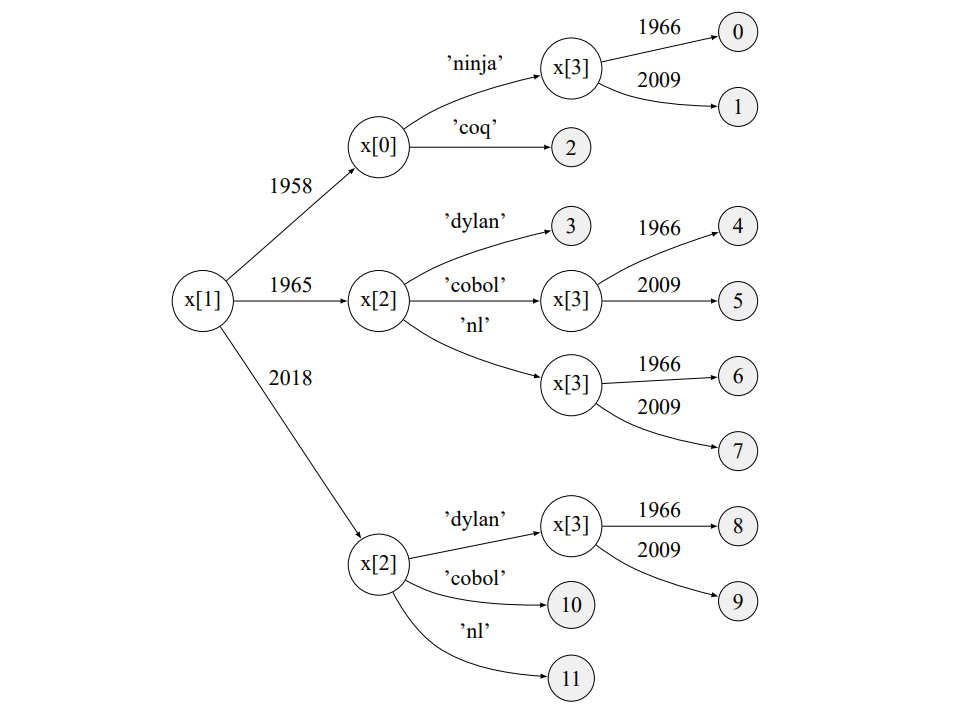
\includegraphics[width=\linewidth]{graph}
			\caption{Дерево решений}\label{pic:2.1}
			%	\vspace{5ex}
		\end{center}	
	\end{figure}
\end{problem}

\begin{nonum}
	Для реализации функции--дерева решений используем условные операторы \textit {if else} для организации вложенного ветвления.
	\begin{lstlisting}
		def solve_tree (list):
			if list[1] == 1958:
				if list[0] == "ninja":
					if list[3] == 1966:
						return 0
					elif list [3] == 2009:
						return 1
				elif list [0] == "coq":
					return 2
			elif list[1] == 1965:
				if list[2] == "dylan":
					return 3
				elif list[2] == "cobol":
					if list[3] == 1966:
						return 4
					elif list[3] == 2009:
						return 5
				elif list[2] == "nl":
					if list[3] == 1966:
						return 6
					elif list[3] == 2009:
						return 7
			elif list[1] == 2018:
				if list[2] == "dylan":
					if list[3] == 1966:
						return 8
					elif list[3] == 2009:
						return 9
				elif list[2] == "cobol":
					return 10
				elif list[2] == "nl":
					return 11
			else:
				return None
	\end{lstlisting}
	\vspace{3ex}
	Примеры вычисления дерева решений $solve_tree$:
	\begin{enumerate}
		\item $solve_tree(['coq', 1958, 'dylan', 2009]) = 2$
		\item $solve_tree(['coq', 1965, 'nl', 1966]) = 6$
	\end{enumerate}
\end{nonum}

\begin{problem}
	 Реализовать функцию--­транскодер
	 	\begin{figure}[h!]
		 	\begin{center}
		 		%\vspace{-5ex}
		 		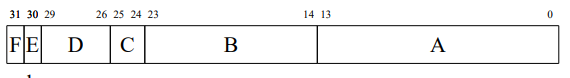
\includegraphics[width=0.8\linewidth]{transcode1}
		 		\caption{Представление исходного числа}\label{pic:2.2.1}
		 		%	\vspace{5ex}
		 	\end{center}	
	 	\end{figure}

 	\begin{figure}[h!]
 	\begin{center}
 		%\vspace{-5ex}
 		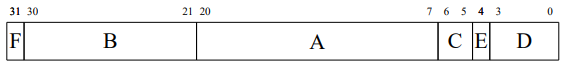
\includegraphics[width=0.8\linewidth]{transcode2}
 		\caption{Представление преобразованного числа}\label{pic:2.2.2}
 		%	\vspace{5ex}
 	\end{center}	
 \end{figure}
\end{problem}

\begin{nonum}
	Для решение данной задачи будем использовать побитовые операции сдвига, логического умножения и логического сложения.
	\vspace{3ex}
	\begin{lstlisting}
	def transcoder (value):
		a = value & 0b11111111111111
		b = (value >> 14) & 0b1111111111
		c = (value >> 24) & 0b11
		d = (value >> 26) & 0b1111
		e = (value >> 30) & 0b1
		f = (value >> 31) & 0b1
		return (a << 7) | (b << 21) | (c << 5) | (d << 0) | (e << 4) | (f << 31)
	\end{lstlisting}
	
	Примеры вычисления функции­транскодер $transcoder$:
	\begin{enumerate}
		\item $transcoder(0x22b67413) = 0x5b3a09c8$
		\item $transcoder(0x3bf48b61) = 0x7a45b0ee$
	\end{enumerate}
\end{nonum}

\begin{problem}
	Реализовать функцию преобразования табличных данных. Входная и выходная таблицы
	заданы в построчной форме, с помощью списков. Заполненные ячейки имеют строковой тип
	данных. Пустые ячейки имеют значение None.
	Над входной таблицей провести ряд преобразований:
	\begin{itemize}
		\item Удалить пустые столбцы
		\item Удалить пустые столбцы
		\item Удалить дубли среди строк
		\item Преобразовать содержимое ячеек по примерам
		\item Отсортировать строки по столбцу №1.
	\end{itemize}
\begin{nonum}
	Для реализации функции--преобразователя таблиц опишем вспомогательные функции, которые будут обрабатывать соответсвующие поля исходной таблицы. Применим функциональные идиомы \textit{map, filter} для удобного обращения со списками.
	\begin{lstlisting}
	def phone_formater (phone_num):
		f = filter(str.isdigit,phone_num)
		clear_phone_num = "".join(f)
		clear_phone_num = clear_phone_num[1:]
		return clear_phone_num
	
	def number_rounder (number):
		return round(number,2)
	
	def date_formater (date):
		date_list = date.split('/')
		short_date = date_list[-1][2:]
		date_list[2] = short_date
		date_list = '.'.join(date_list)
		return date_list
	
	def erase_none (mylist):
		return list(filter(lambda el: not(el is None),mylist))
	
	def unique (not_typed_list):
		n = []
		for i in not_typed_list:
			if i not in n:
				n.append(i)
		return n
		
	def table_formater (table):
		# table is list of list of string
		def pretty_row (row):
			# row is a list of string
			clean_row = erase_none(row)
			clean_row[0] = phone_formater(clean_row[0])
			clean_row[1] = number_rounder(float(clean_row[1]))
			clean_row[2] = int(1) if bool(clean_row[2]) else int(0)
			clean_row[3] = date_formater(clean_row[3])
			return clean_row
		answer = list(map(pretty_row,table))
		answer = list(map(lambda row: list(map(str,row)),answer))
		answer = unique(answer)
		answer.sort(key = operator.itemgetter(0,1))
		return answer 
	\end{lstlisting}
	Примеры табличных преобразований:
	\begin{figure}[h!]
		\begin{center}
			%\vspace{-5ex}
			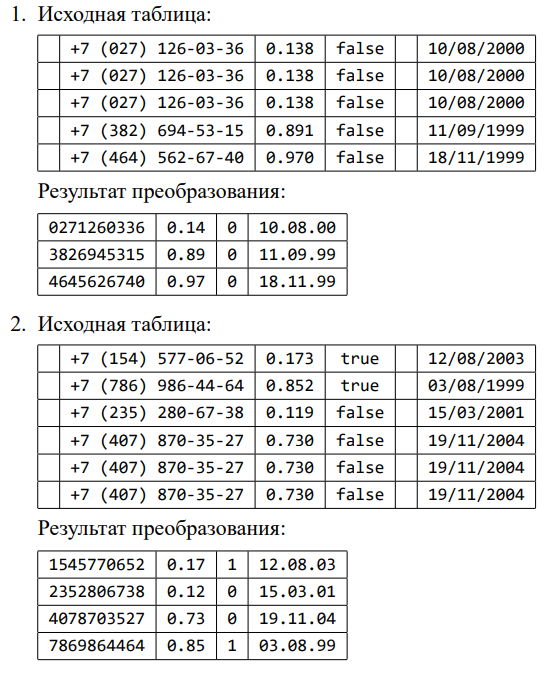
\includegraphics[width=0.8\linewidth]{table-inp-outp}
			\caption{Форматирование таблиц}\label{pic:2.3}
			%	\vspace{5ex}
		\end{center}	
	\end{figure}
\end{nonum}
\end{problem}
\section{Вывод}
В ходе выполнения данной практической работы были приобретены знания по использованию условных и циклических операторов, математических функций в языке программирования Python. Полученные знания были применены на практике.
\end{document}

